 %\title{Landscape Brochure Template}
 % This example is from http://www.ctan.org/tex-archive/macros/latex/contrib/flowfram/
 

\documentclass[a4paper, 11pt]{report}
\usepackage{amsmath}
\usepackage[landscape,margin=1in]{geometry}
\usepackage{color}
\usepackage{flowfram}
\usepackage[colorlinks]{hyperref}
\usepackage{indentfirst}
\usepackage{graphicx}
\usepackage{csquotes}
\usepackage{setspace}

\newtheorem{mydef}{Definicão}
\newtheorem{proof}{Demonstração}
\renewcommand{\baselinestretch}{1.2} 

\newenvironment{myboxed}
    {
        \begin{center}
        \begin{tabular}{p{0.7\textwidth}}
        \hline\
    }
    { 
        \\\hline
        \end{tabular} 
        \end{center}
    }


\renewcommand{\familydefault}{cmss}

\adjustheight{\textheight}

\onecolumninarea[1-100]{0.7\textwidth}{\textheight}{0.3\textwidth}{0pt}
%\twocolumninarea[>3]{0.8\textwidth}{\textheight}{0.52\textwidth}{0pt}


\newdynamicframe{0.2\textwidth}{0.8\textheight}{0pt}{0pt}[left]

\dfchaphead*{left}
\renewcommand{\DFchapterstyle}[1]{%
\raggedright\Huge\slshape\MakeUppercase{#1}\par}

\vtwotone[1]{0.3\paperwidth}{[cmyk]{0.37,0,0.07,0.50}}{backleft}%
{0.7\paperwidth}{[cmyk]{0.37,0,0.15,0.32}}{backright}

\vtwotonetop{1cm}{0.3\paperwidth}{[cmyk]{0.37,0,0.07,0.50}}{topleft}%
{0.7\paperwidth}{[cmyk]{0.37,0,0.15,0.32}}{topright}

\newstaticframe[1]{0.2\textwidth}{0.25\textheight}{0pt}{0pt}[logo]

\pagestyle{empty}

\renewcommand{\chapterfirstpagestyle}{empty}

\newdynamicframe[>1]{\textwidth}{\headheight}{0pt}{-\footskip}[footer]

\setdynamiccontents*{footer}{%
Prof. Dr. Reginaldo Leão  \hfill
GESESC, IFMG - Arcos\hfill
pag \thepage\ de \pageref*{lastpage}}

\newcommand{\env}[1]{\texttt{#1}}
\newcommand{\cmdname}[1]{\texttt{\symbol{92}#1}}
\newcommand{\meta}[1]{\textnormal{\textless\textit{#1}\textgreater}}

\begin{document}

\setstaticcontents*{logo}{\sffamily{\Huge\slshape IFMG\&GESESC} \\ 
Instituto Federal de Minas Gerais  ---\\
Grupo de Estudos em Sistemas Energéticos e Simulação Computacional.}

{\noindent
\slshape\Huge\MakeUppercase{FÍSICA I: Mecânica \\} 
Notas de Aulas :: {Versão 2 - Agosto de 2021} \par
\vskip0.3in
\noindent\large{Prof. Dr. Reginaldo Leão} \\
}\date{\today}

\chapter{Medidas e Unidades}
\begin{center}
    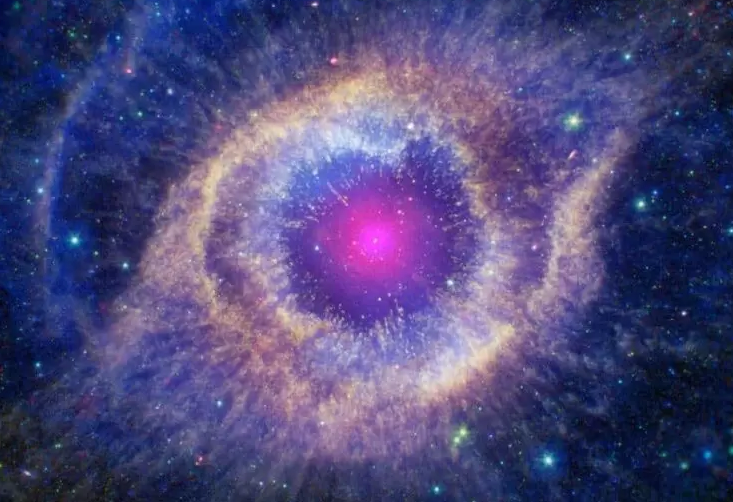
\includegraphics[scale=.4]{img/nebhelix.png}

    {\footnotesize Nebulosa Hélix, concepção artística baseada em dados 
    observacionais - Fonte: NASA}
\end{center}

\section{Introdução}
A Física é uma das Ciências Naturais mais fundamentais que existem; por 
fundamental me refiro ao nível de detalhamento de seu objeto de estudo. Enquanto 
a Química se ocupa "principalmente" das transformações da matéria em nível 
molecular  - quando a agregação das partículas fundamentais que compõem 
a matéria já é extremamente complexa - a Biologia, se ocupa principalmente dos 
organismos sua complexidade e relações - quando a organização molecular se dá 
de maneira tal que pode ser caracterizada como vida. A Física, por outro lado, se
debruça sobre os entes que permitem tais estruturações e vai além; extrapola 
suas inferência para explicar tudo o mais que nos rodeia, a começar do tempo e o
espaço, a matéria, seus distintos estados de agregação, as forças e relações 
quânticas que permitem suas transformações, sua aglutinação gravitacional e a 
formação dos corpos celestes, o próprio ciclo de vida dos elementos componentes
da matéria, constantemente fundidos e destruídos no coração de estrelas jovens e 
velhas, a organização e complexidade das galáxias e o cosmos.

Embora o ser humano seja naturalmente um animal questionador, só foi possível 
alcançar o atual status de desenvolvimento científico e tecnológico,
graças à sua capacidade de observar algo de forma 
sistemática, registrá-lo e organizá-lo logicamente, de modo tal que o permitisse
sugerir inferências fundamentadas, questionar o observado e 
buscar respostas consistentes. 

Ao longo da história, as mentes mais curiosas da humanidade fizeram esse 
percurso de construção do conhecimento de muitas formas distintas e não 
lineares. Alguns de forma mais consistentes, outros menos; variações daquilo que
atualmente chamamos \emph{Método Científico}, um conjunto de regras por meio
das quais podemos construir novos conhecimentos de uma forma satisfatoriamente 
confiável. 

Ainda que, o Método Científico seja quase sempre atribuído a Isaac Newton, ou as
vezes a Galileu Galilei, sua criação não pode ser de fato conferida a um único 
autor. O pensamento greco-ocidental, os lastros históricos do conhecimento 
científico de egípcios, sumérios e mesopotâmicos, o pensamento filosófico 
racionalista e determinista e mesmo contribuições recentes como a Teoria da 
Complexidade de Edigar Morin, foram fundamentais para compor a complexidade e o
nível de especialidade e precisão da ciência moderna.

No entanto, a despeito de todo o arcabouço conceitual por trás do método, é 
possível sugerir que o átomo do método científico provavelmente seja a 
\emph{medida}. 

\section{Medidas Físicas}
Na Física, a ação de medir deve ser entendida como o ato de se determinar um 
valor \textbf{satisfatóriamente preciso} para uma \emph{grandeza física}.

Note que na definição anterior, dois conceitos foram introduzidos:
\begin{itemize}
    \item[\emph{i)}] o conceito de precisão satisfatória;
    \item[\emph{ii)}] e o conceito de grandeza física
\end{itemize}

O primeiro deles está associado a impossibilidade de se medir com precisão total
o valor de uma grandeza. Em outras palavras \emph{é impossível determinar o 
valor verdadeiro de uma grandeza física.} 

Esta impossibilidade se deve ao fato de que medir algo, significa compará-lo com
um determinado padrão. Quando se mede a distância entre duas cidades, o que se 
faz é comparar o espaço entre elas (medido segundo algum critério previamente
determinado, como distância rodoviária ou geodésica) com o padrão quilômetro, 
por exemplo. Logo se quantifica a distância de interesse como múltipla ou 
submúltipla deste padrão previamente estabelecido.

O próprio quilômetro ($km$) é na verdade um múltiplo de uma unidade fundamental 
do Sistema Internacional de Unidades (SI), o metro ($m$). Ainda que exista uma 
definição histórica bastante curiosa para essa grandeza \footnote{Pesquise pela 
"históriado metro" para saber mais}, fisicamente, a unidade métrica é aceita 
como a distância percorrida pela luz em uma fração de tempo igual a 
$1/299 792 458$ segundos. A propósito, a unidade de tempo segundos ($s$) também 
é uma unidade fundamental do SI. 

Deste modo, medir a distância entre duas cidades, significa comparar tal
distância a um conjunto de unidades quilométricas linearmente justapostas a que
dá-se o nome de "escala quilométrica". Uma medida inteira nesta escala hipotética
está condicionado, ao fato de que os pontos que marcam as limites da distância 
medida, coincidam com os extremos de cada unidade quilométrica da escala, 
configuração esta cuja a probabilidade de ocorrência é infinitesimal já que a 
cada 01 km apenas um único ponto atende a tal condição. 

Par descrever qualquer outra medida que não seja inteira, recorre-se aos 
submúltiplos do escala original, o metro por exemplo, \emph{a o que se denomina 
aumento de resolução}. Deste modo a escala quilométrica passa a ser subdividida 
em 1000 partes iguais,  cada qual com 1 $m$ de extensão. No entanto, retorna-se 
certamente na mesma dificuldade de medida, já que a cada metro apenas um ponto 
é capaz de expressar um valor inteiro de medida nessa escala. Medidas não 
inteiras poderiam ser expressas como a centésima parte do metro o centímetro 
($cm$) e em seguida milímetros e assim sucessivamente \emph{ad infinitum}. 

Como se vê, a redução da escala incrementa a precisão de uma medida apenas até
certo nível, já que independentemente daquela utilizada, o problema da 
indeterminação do valor absoluto da medida se mantém, considerando que apenas
o conhecimento de um determinado ponto dentre outros infinitos atenderia essa 
premissa. Além disto, o incrementos sucessivos na resolução da escala, 
simultaneamente potencializa a questão da \emph{acuidade}, que é nível de 
capacidade que um determinado sensor - um ser humano usando o sentido da visão, 
por exemplo - possui de perceber a distinção entre múltiplas medidas. Donde se
chega a ideia de \emph{precisão satisfatória} para a medida sendo realizada. 
\newline 
\begin{myboxed}
    \textbf{IMPORTANTE:}
    \emph{
        Deve-se estabelecer de forma planejada e antecipada, o nível de precisão 
        desejado para uma medida, e só então selecionar o instrumento e 
        a metodologia ideal para a tomada desta.
    }
\end{myboxed}

\subsection{Incerteza de Medidas}
Obviamente, quando se estabelece uma precisão limite, não se pode apenas
desprezar a imprecisão associada, de modo tal que é preciso tratar a 
\textbf{\emph{incerteza}} ($\sigma$) associada à medida. Assim para a expressão 
correta de uma medida, é preciso informar simultaneamente o valor da leitura e 
esse valor de incerteza. 

A incerteza representa o intervalo de confiança de uma leitura através de um 
intervalo finito e não nulo representado nas formas das Equações 
\ref{Eq:med_incert_simetrica} e \ref{Eq:med_incert_assimetrica}

\begin{equation}
    m = M \pm \sigma
    \label{Eq:med_incert_simetrica}
\end{equation}
\begin{equation}
    m = M^{+\sigma'_{M_+}}_{-\sigma''_{M_-}}
    \label{Eq:med_incert_assimetrica}
\end{equation}

A Equação \ref{Eq:med_incert_simetrica} representa a incerteza simétrica em 
torno da leitura ($M$), ao passo que a Equação \ref{Eq:med_incert_assimetrica}
representa a incerteza assimétrica em torno de $M$. Ou seja $M$ pode variar 
entre $M + \sigma$ e $M - \sigma$ na Equação \ref{Eq:med_incert_simetrica} e 
$M + \sigma'$ e $M - \sigma''$ na Equação \ref{Eq:med_incert_assimetrica}.

São muitos os métodos para o cálculo de $\sigma$, para a avaliação da precisão 
e seleção do número de algarismos significativos, e dependem, dentre outras 
coisas, do instrumento utilizado, da metodologia e do número de fontes de erros.
Os detalhes deste tipo de análise merecem considerações mais pormenorizadas e 
uma discussão mais elaborada, e só serão tratados desta forma em outra obra 
complementar a essa. 

No entanto, algumas convenções simples podem ser adotadas.

\subsubsection{Convenções sobre incertezas e algarismos significativos}
Algarismos significativos \emph{são os dígitos numéricos de um valor que 
possuem significado}, exatamente por isso podem ser utilizados para se 
representar, dentre outras coisas, estimativas da incerteza de uma medida.

Suponha uma régua semelhante à da Figura \ref{Img:reguaescolar}, 
graduada em milímetros ($mm$). Ao ser usada para medir o 
objeto, a leitura obtida é certamente 63 $mm$, porém há alguma 
dúvida sobre o comprimento do objeto que se estende para além deste ponto. 

\begin{staticfigure}
    \centering
    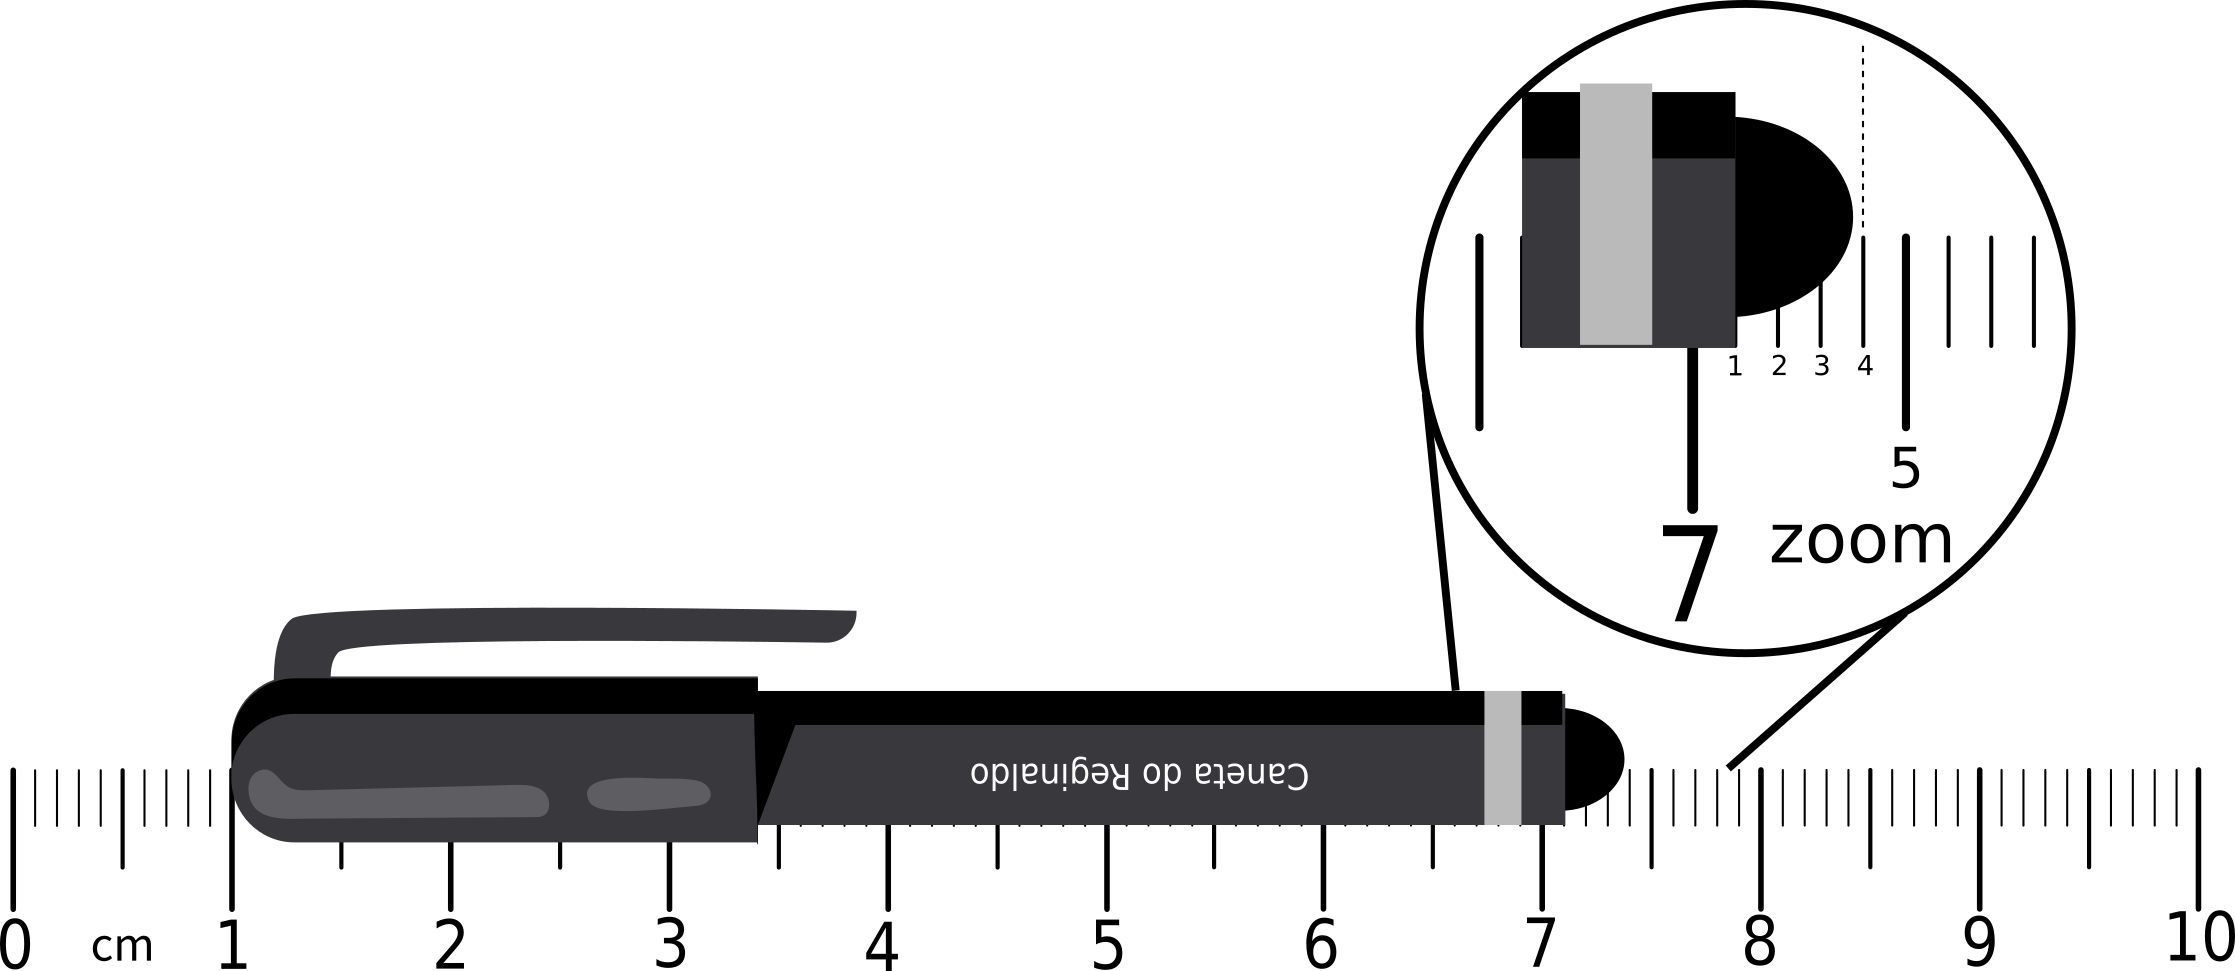
\includegraphics[scale=.45]{img/reguaescolar.png}
    \caption{\footnotesize Régua graduada.}
    \label{Img:reguaescolar}
\end{staticfigure}

Observando mais atentamente a região de \emph{zoom} na imagem, é possível 
observar que a extremidade da caneta está além do terceiro milímetro após a 
marcação de 7 $cm$ na escala. Alguns avaliarão essa medida residual como 
como $7/10 \: mm$, provavelmente a maioria como $8/10 \: mm$ e
alguns ainda avaliarão como $9/10 \: mm$. De fato, 63,7 $mm$, 63,8 $mm$ e 
63,9 $mm$ \textbf{são todas medidas válidas, igualmente certas e igualmente 
erradas}.

A leitura 63 corresponde ao valor de $M$ na Equação 
\ref{Eq:med_incert_simetrica}, mas qual a incerteza dessa medida ? 

Em instrumentos analógicos, como é o caso da escala graduada, a convenção mais 
comum adota a incerteza como sendo igual a metade da \textbf{precisão} do 
instrumento. A escala da Figura \ref{Img:reguaescolar} tem precisão de 1 $mm$, 
portanto, a incerteza de medidas em escalas como essa é de 0,5 $mm$. 
Considerando um leiturista que sugerisse 63,8 $mm$ para o tamanho da caneta, 
o valor da medida seria $m = 63,8 \pm 0,5$ $mm$.

Na leitura em questão a convenção demonstrada na Figura \ref{Img:algsign} é 
adotada para a identificação dos algarismos significativos. 

\begin{staticfigure}
    \centering
    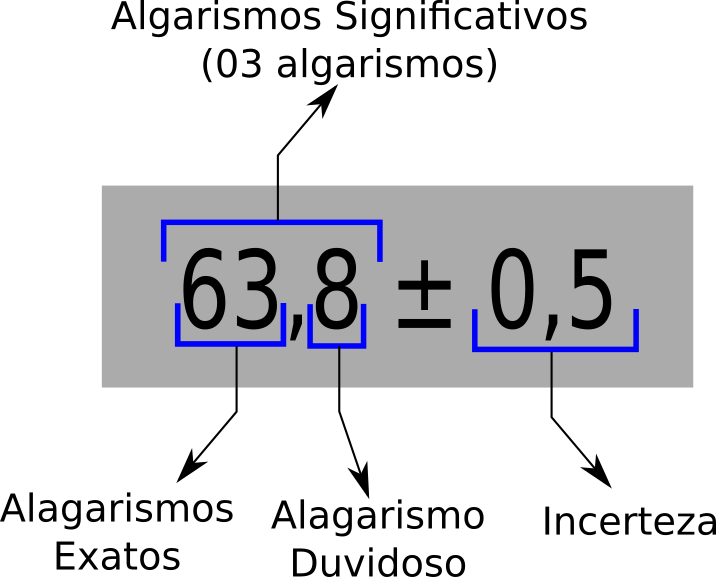
\includegraphics[scale=.55]{img/algarismossig.png}
    \caption{\footnotesize Algarismos de uma leitura.}
    \label{Img:algsign}
\end{staticfigure}

Algarismos exatos são aqueles que se pode determinar com certeza absoluta na 
leitura da escala, já o algarismo duvidoso, será sempre aquele que pode 
suscitar dúvida entre diferentes leituristas. Como o algarismo duvidoso 
carrega inexatidão, \emph{não faz sentido que qualquer leitura possua mais do que 
apenas um algarismo deste tipo}.

Outra convenção importante que geralmente é adotada na falta de algo mais 
preciso, é a forma de determinação da incerteza de uma medida na qual este 
valor não foi explicitamente declarado. Nestes casos, \emph{é comum se adotar a 
incerteza como sendo a metade do valor unitário do menor alagarismo exato}.

\begin{myboxed}
    \textbf{IMPORTANTE:}

    \emph{
    1. Qualquer medida de uma determinada grandeza deve possuir apenas um 
    algarismo duvidoso.
    }

    \emph{
    2. A incerteza de medidas para as quais este valor não foi explicitamente 
    declarado, deve ser assumida como sendo igual à metade do valor unitário do
    menor algarismo significativo exato.
    }
\end{myboxed}

\subsubsection{O problema do algarismo zero (0)}
Zeros que são colocados em um número para posicionar o separador decimal, jamais
devem ser considerados algarismos significativos. Estes casos são melhores 
identificados na composição de medidas expressas em unidades de medida 
diferentes daquelas dos instrumentos em que foram determinadas.

Suponha, por exemplo, uma balança comercial com precisão de 0,1 quilogramas 
($kg$), que tenha feito uma leitura de 2,5 $kg$. Quando este valor é expresso em
gramas - uma unidade de medida distinta daquela original da balança -, então a 
leitura ficaria 2500 gramas ($g$). Note que no número 2500, os zeros a direita, 
não tem significado pois a balança não possui tal precisão, portanto não são 
significativos e só existem para possibilitar a ocorrência do ponto decimal 
em uma posição correspondente a unidade grama.

De forma semelhante, se uma balança graduada em gramas mede 20 $g$ e o 
usuário, desejando expressar esse valor em $kg$ o escreve como 0,020 $kg$, os 
zeros a esquerda não são significativos, pois só foram introduzidos para 
possibilitarem a colocação do separador decimal na casa deciaml correspondente 
à unidade de medida de massa desejada. Este tipo de técnica é bastante comum na 
Física, quando se precisa compatibilizar diferentes unidades de medida de uma 
mesma grandeza, ou se operar com grandezas distintas compondo uma unidade 
derivada desejada, ou mesmo para a compatibilização de unidades com constantes 
físicas. 

Para evitar a dificuldades no acompanhamento dos algarismos significativos, é 
bastante recomendável que as medidas e constantes físicas sejam expressas como 
potências de 10 em Notação Científica. 

\subsubsection{Notação Científica}
A notação científica é um pelo qual valores são expressos por meio de 
potências de dez ($10^{n}$) multiplicadas pela mantissa ($\mathcal{M}$) do valor
 que se deseja representar, somada à incerteza deste valor, conforme mostrado pela 
 Equação \ref{Eq:pot_dez}.

 \begin{equation}
     m = (\mathcal{M} \pm \sigma) \cdot 10^n
     \label{Eq:pot_dez}
 \end{equation}

É também convencionado que o valor de $\mathcal{M}$ deve estar em um intervalo 
entre $1 \leq \mathcal{M} < 10$.

Para compreender melhor o uso do recurso, vamos expressar a leitura da régua 
para o tamanho da caneta em notação científica. Como a medida foi de 
$63,8 \pm 0,5 \: mm$, deve-se multiplicar o valor por $10^{-1}$ para que a 
mantissa esteja entre $1 \leq \mathcal{M} < 10$.

\begin{myboxed}
    \textbf{SEÇÃO DE CÁLCULOS:}

    $
        (63,8 \pm 0,5) \cdot 10^{-1} = (6,38 \pm 0,05) \cdot 10^{-1}
    $
\end{myboxed}

Neste caso, a vantagem do uso de notação científica não é tão aparente, porém, 
no exemplo da seção anterior, quando o significado dos zeros na leitura 
$2500 \: g$ foi discutido, a forma de $\mathcal{M}$ indica exatamente o número 
de algarismos significativos no valor.

\begin{myboxed}
    \textbf{SEÇÃO DE CÁLCULOS:}

    $
        (2500 \pm 100) \cdot 10^{-3} \: g = (2,5 \pm 0,1) \cdot 10^{-3} \: g
    $
\end{myboxed}

É possível notar que a mantissa possui exatamente dois algarismos 
significativos, além disso, deve ser observado que neste instrumento em 
específico, a incerteza foi assumida como sendo de $100 \: g$. \emph{Em 
instrumentos digitais a incerteza é fornecida pelo fabricante ou convencionada 
como sendo sua resolução}.

\subsubsection{Algarismos Significativos nas Operações Matemáticas 
Básicas}

Quando grandezas são operadas matematicamente, deve-se determinar uma convenção 
para o tratamento do número de algarismos significativos e incertezas de 
medidas. Os métodos de tratamento da propagação das incertezas através das 
operações matemáticas são um pouco mais complexos e não serão tratados neste 
tópico introdutório. Todavia, as convenções para o cuidado com o número de 
algarismos significativos são bastante simples, conforme pode ser visto na lista
abaixo.

\begin{myboxed}
    \textbf{Convenções para determinação do número de algarismos significativos 
    nas operações matemáticas básicas.}

    \begin{enumerate}
        \item \textbf{SOMA E SUBTRAÇÃO:} O número de \emph{casas decimais} no 
        resultado deve ser igual ao número da menor quantidade de casas dentre 
        aquelas presentes nos termos da operação.
        \item \textbf{MULTIPLICAÇÃO E DIVISÃO:} O número de \emph{algarismos 
        significativos} no resultado deve ser igual ao número da menor 
        quantidade de algarismos significativos dentre aqueles presentes nos 
        termos da operação.
        \item \textbf{ESTIMATIVAS:} Todos os resultados estimados devem possuir
        apenas um algarismo significativo, segundo sua órdem de grandeza. 
    \end{enumerate}
\end{myboxed}

Quando arredondamento se fizerem necessários para o atendimento às regras 
anteriores, então a seguinte convenção deve ser utilizada.

\begin{myboxed}
    \textbf{Regras para arredondamento}

    Após a seleção do total de dígitos conservados - aqueles que parmanecerão no 
    valor - segundo as regras de determinação do número de algarismos 
    significativos, deve-se verificar se:

    \begin{itemize}
        \item o primeiro algarismo abandonado for maior que 5, ou sendo 5 e 
        o seguinte qualquer que não seja 0, o último 
        dígito conservado deve ser acrescido de uma unidade  
        (e.g. $1,7|6 \rightarrow 1,8| $ ou $1,7|51 \rightarrow 1,8| $); 
        \item o primeiro algarismo abandonado for menor que 5, o último 
        dígito conservado não deve ser alterado 
        (e.g. $1,7|3 \rightarrow 1,7| $);
        \item  o primeiro algarismo abandonado for igual a 5 seguido de um 
        dígito zero, o último dígito conservado deve ser acrescido 
        de uma unidade, se for ímpar, e mantido, se for par.
        (e.g. $ 1,7|50 \rightarrow 1,8| $ ou $ 1,6|50 \rightarrow 1,6| $); 
    \end{itemize}
\end{myboxed}

\subsubsection{Ordens de Grandezas e Estimastivas}

\begin{flushright}
    "A \emph{Via-Láctea} é uma galáxia espiral com pouco mais \\
    de $10^5$ anos luz de diâmetro, idade de $10^{10}$ anos \\
    terrestres e $10^{11}$ estrelas vivas." 
\end{flushright}

Ao ler o texto anterior, não é difícil inferir que os dados informados são todos
\textbf{estimativas} dos respectivos valores reais, impossíveis de serem 
determinados precisamente no atual estágio de desenvolvimento científico. 

Os valores usados para representar as grandezas mencionadas são todos exemplos de 
estimativas dadas como \textbf{ordens de grandeza}. 

Uma ordem de grandeza, é uma potência de dez (\emph{atenção para não confundir
o conceito com o de notação científica}) usada para expressar com confiabiliade 
aceitável, um valor cuja a expressão precisa seja impossível, muito dispendiosa, 
ou desnecessária. \emph{A potência selecionada para este propósito, deve ser a mais
próxima do valor que se está estimando.} 

As dimensões de nossa galáxia, o número de átomos de carbono presentes em um 
organismo vivo e o número de elétrons livres em uma unidade métrica cúbica de 
um condutor elétrico, são todos exemplos de grandezas que podem ser 
satisfatoriamente representadas por uma órdem de grandeza. 

Vejamos um exemplo.

\begin{myboxed}
    \textbf{EXEMPLO - Estimando o número de átomos de carbono no corpo humano.}

    No livro 
    \emph{What Do You Think You Are? The science of what makes you you}, de 
    Brian Clegg, o autor estima o fração mássica média de átomos de carbono no 
    organismo humano como algo próximo de 18\%. 

    Sabendo disto, estime a ordem de grandeza do número de átomos de carbono 
    em um ser humano com massa de 70 kg.

    \textbf{SOLUÇÃO:}

    Se 18\% dos 70 kg da massa corpórea na situação proposta forem átomos de 
    carbono ($C$), então tem-se uma massa de:
    
    $$
        m_C = 70 \cdot 0,18 \approx 13 kg
    $$

    Considerando a massa do elemento C, dada a abundância isotópica, como de 
    aproximadamente $12 \: g.mol^{-1}$. Então em $1,3 \cdot 10^4 \: g$
    \emph{
        (Note aqui a utilização da notação científica para adequação do número de
        algarismos significativos.)
    }
    tem-se:

    $$ 
        M_{molar} = \frac{m}{N_{mols}} \rightarrow 
        12 = \frac{1,3 \cdot 10^4}{N_{mols}} \rightarrow 
        N_{mols} \approx 1,1 \cdot 10^3 mols
    $$

    Agora considerando a constante de Avogadro ($N_A$) como $6,0 \cdot 10^{23}$, podemos
    determinar o número de átomos $N_C$.

    $$
        N_C = {N_{mols}}\cdot{N_A} = {1,1 \cdot 10^3}\cdot{6,0 \cdot 10^{23}} 
        \rightarrow N_C \approx 6,6 \cdot 10^{26}  \approx 10^{27} 
        \text{ átomos de carbono}.
    $$
 
\end{myboxed}

Alguns valores como 5, 50, 500... geralmente costumam gerar alguma confusão 
quando precisam ser expressos como ordens de grandeza, no entanto a confusão é 
apenas aparente. Note na sequência abaixo que o número cinco não é um ponto 
equidistante às potências de 10 mais próximas, mas sim o  valor 5,5.

$$
    ...10^0, 2, 3, 4, \text{\LARGE 5}, 6, 7, 8, 9, 10^1...
$$

Deste modo, utilizaremos como critério de seleção da potência de dez a seguinte
regra:

\begin{myboxed}
    \textbf{Regras para a seleção da potência de dez em estimativas de órdens
    de grandeza.}

    Valores que quando expressos na forma de notação científica sejam menores
    5,5 terão ordem de grandeza igual à potência de dez da notação, do contrário
    terão ordem de grandeza igual à potência de dez imediatamente superior.
\end{myboxed}

Existem outras convenções para este propósito, no entanto, por questão de 
simplicidade e por tratar-se de disciplina introdutória, manteremos este padrão
por todo o semestre. 

\begin{statictable}
    \caption{Tabela de prefixos.}
    \label{Tab:prefixosOG}
    \begin{tabular}{lcc}
        \textbf{Prefixo} & \textbf{Símbolo} & \textbf{Ordem de Grandeza} \\
        \hline
        Femto	& $f$	& $10^{-15}$ \\
        Pico	& $p$	& $10^{-12}$ \\
        Nano	& $n$	& $10^{-9}$ \\
        Micro	& $\mu$	& $10^{-6}$ \\
        Mili	& $m$	& $10^{-3}$ \\
        Centi	& $c$	& $10^{-2}$ \\
        Deci	& $d$	& $10^{-1}$ \\
        \hline
    \end{tabular}
    \begin{tabular}{lcc}
        \textbf{Prefixo} & \textbf{Símbolo} & \textbf{Ordem de Grandeza} \\
        \hline
        Deca	& $da$	& $10^{1}$ \\
        Hecto	& $h$	& $10^{2}$ \\
        Quilo	& $k$	& $10^{3}$ \\
        Mega	& $M$	& $10^{6}$ \\
        Giga	& $G$	& $10^{9}$ \\
        Tera	& $T$	& $10^{12}$ \\   
        Peta    & $P$   & $10^{15}$ \\
        \hline
    \end{tabular}\\
\end{statictable}

Algumas vezes as ordens de grandeza, ou mesmo as grandezas propriamente ditas, 
podem ser expressas por meio de abreviações representativas de sua magnitude. 
Quando dizemos \emph{quilômetro} representado por $km$, utilizamos o prefixo 
quilo (\emph{kilo}), junto à unidade metro, significando que esta unidade 
equivale a 1000 vezes o valor unitário do metro. Já quando utilizamos milímetro
$mm$, adicionamos o prefixo mili à unidade de metro, dizendo que esta unidade se
refere à milésima parte do metro. Na Tabela \ref{Tab:prefixosOG}, podem ser 
vistos os prefixos mais usuáis para esse propósito.

\subsection{Unidades e Grandezas}

Uma das principais tarefas da Ciência Física é propor modelos explicativos, e 
as vezes preditivos, para um determinado fenômeno natural. Como dito
anteriormente, a Física, e todas as ciências legítimas, utilizam um conjuto de 
regras e protocolos para coletarem informações sobre um fenômeno ou objeto 
estudado de forma mais consistente e segura. As ciências naturais e exatas, 
geralmente, valem-se de medidas quantitativas para realizar tal tarefa. 

Uma medida, nada mais é que a quantificação de uma grandeza; que por sua vez, 
deve ser entendida como uma característica bem definida e delimitada do objeto
ou fenômeno estudado. A Física, como ciência fundamental, se ocupa, na grande 
maioria das vezes, de grandezas igualmente fundamentais, ou seja, 
capazes de descrever bem, pelo menos do ponto de vista clássico \footnote{
    Pesquise sobre as diferenças entre a Física Clássica e Moderna.
}, o tempo, o espaço e a matéria.

Essas grandezas fundamentais, tal como foram historicamente definidas e/ou 
padronizadas, não podem ser expressas a partir de outras grandezas, também por 
isso são chamadas \textbf{grandezas fundamentais}. São elas o 
\emph{i)} \textbf{comprimento}, cuja unidade padrão no Sistema Internacional de
Unidades (SI) é o metro; \emph{ii)} o \textbf{tempo}, cuja unidade padrão no SI
é o segundo; \emph{iii)} a \textbf{massa}, cuja a unidade padrão é o quilograma
e a \emph{iv)} \textbf{carga elétrica}, cuja a unidade padrão para a medida é 
Coulomb ($C$). Todas as unidade mecânicas clássicas podem ser, de alguma forma, 
obtidas a partir das três primeiras grandezas fundamentais. 

Considerando, a existência das grandezas fundamentais, comprimento, tempo e 
massa, pode-se introduzir o conceito de dimensão. Na Física, a palavra dimensão, 
significa a natureza física de uma determinada quantidade. As grandezas 
fundamentais, estabelecem as dimensões físicas mais simples, o comprimento, 
possui dimensão $L$, a massa $M$, o tempo $T$ e a carga elétrica $Q$. Note que
os símbolos $L$, $M$, $T$ e $Q$, não denotam nenhuma unidade de medida 
específica, mas sim uma grandeza fundamental. Daí podemos derivar outras 
grandezas. A área, por exemplo, tem dimensão ($L \times L = L^2$) independente 
de sua unidade ser o $m^2$ ou o $ft^2$
\footnote{
    Um pé $ft$ (do inglês \emph{foot}) equivale a $0,3048\:m$.
}. A velocidade, por sua vez é uma grandeza cuja a dimensão é $\frac{L}{T}$, 
independentemente de sua unidade de medida. 

Para a determinação da dimensão de uma grandeza derivada, como a velocidade ou 
área, por exemplo, se utiliza o recurso da análise dimensional. 

\subsubsection{Análise Dimensional}
Quando se trabalha com grandezas cujas as dimensões são desconhecidas, é
necessário se proceder uma análise dimensional para determiná-las. Este tipo de 
análise, permite, dentre outras coisas, a determinação e verificação da correção
de unidades de medida e equacionamento utilizado. 

Nestes casos, nos referimos a dimensão de uma grandeza $a$ por meio do símbolo
$[a]$. Suponha que um experimento determinou que a posição de um corpo é 
diretamente proporcional à metade do quadrado do tempo de medida conforme a 
Equação \ref{Eq:prop_pos}.

\begin{equation}
    x \propto \frac{1}{2} t^2
    \label{Eq:prop_pos}
\end{equation}

Para converter essa proporcionalidade em igualdade precisamos multiplicá-la por 
uma constante $k$ de tal forma que a Equação \ref{Eq:prop_pos} fica na forma 
dada pela Equação \ref{Eq:igual_pos}.

\begin{equation}
    x = k \cdot \frac{1}{2} t^2
    \label{Eq:igual_pos}
\end{equation}

No entanto, qual o significado físico de $k$? A melhor forma de responder tal 
pergunta é por meio de uma análise dimensional. Conforme mostrado no exemplo 
abaixo. 

\begin{myboxed}
    \textbf{EXEMPLO - Determinando o significado de uma constante desconhecida.}

    Determine a dimensão de $k$ na equação $x = k \cdot \frac{1}{2} t^2$, 
    onde $[x] = L$ e $[t] = T$

    \textbf{SOLUÇÃO:}

    Substituindo os símbolos das grandezas por suas respectivas dimensões tem-se
    $$
        L = [k] \cdot T^2
    $$
    
    Note que a fração $\frac{1}{2}$ foi omitida pois números são adimensionais. 

    Então:

    $$
        [k] = \frac{L}{T^2}
    $$

    Logo $k$ é uma grandeza dimensional, então deve ter significado físico, 
    neste caso, a dimensão $L/T^2$ correspondente a grandeza cinemática 
    aceleração. Logo as observações do exemplo, conduzem a equação:

    $$
        x(t) = \frac{1}{2} a t^2
    $$
\end{myboxed}

\begin{myboxed}
    \textbf{EXEMPLO - Determinando a unidade de Força em termos de unidades
    fundamentais.}

    Sabendo que a Segunda Lei de Newton, dentre outras formas, pode ser 
    enunciada como $F = m \: a$, então determine a unidade de força (N) em 
    termos de unidades de grandezas fundamentais no SI.

    \textbf{SOLUÇÃO:}
    $$
    [F] = [m] \: [a] \rightarrow
    [F] = kg \cdot \frac{m}{s^2}
    $$

    Logo $1 \: N = 1 \: kg \cdot \frac{m}{s^2}$.

\end{myboxed}

\subsubsection{Grandezas escalares e vetoriais}

Além da complexidade dimensional de uma grandeza física, elas podem ser 
classificadas também segundo seu caráter escalar ou vetorial. Uma grandeza 
escalar é completamente expressa por sua magnitude (parte numérica) e unidade
de medida, já as grandezas vetoriais só podem ser completamente descritas 
quando expressas por magnitude, unidade de medida, direção e sentido. 

As grandezas escalares são operadas matematicamente como qualquer escalar 
matemático, porém as vetorias estão sujeitas ao mesmo rigorismo matemático 
dos vetores estudados na Geometria Analítica e Álgebra Linear. 

O terceiro capítulo destas notas de aula, apresentará uma revisão bastante 
contextualizada e rigorosa dos métodos de operação com grandezas físicas
vetoriais.

\chapter{CINEMÁTICA DO PONTO MATERIAL}

\section{Cinemática Retilinear}
\subsection{Difinições Fundamentais}
As variáveis, jargão e conceitos utilizados para o estudo da Cinemática e 
Dinâmica são bem estabelecidas, conhecê-las é fundamental para a completa 
compreensão de toda a discussão proposta na disciplina. 

Os conceitos mais fundamentais são os de \textbf{Ponto Material $P$}, 
\textbf{Posição $\vec{r}$} e \textbf{Deslocamento $\Delta \vec{r}$}.

\subsubsection*{Ponto Material}
\begin{mydef}
    O termo Ponto Material $(P)$ refere-se a um ponte geométrico que representa
    o centro de massa de um corpo e onde estaria virtualmente concentrada toda a massa do 
    mesmo corpo. 
\end{mydef}

A utilização de modelos físicos nos quais os corpos sejam simplificados como pontos materiais
deve ser restrita a casos nos quais as dimensões do corpo, ou sua rotação,
não influam sobre a análise mecânica pretendida. Em Física I, trabalharemos 
principalmente com problemas desta natureza. 

\subsubsection*{Vetor Posição}
\begin{mydef}
    A posição, ou como é mais comumente denominado, o Vetor Posição, 
    $(\vec{r})$ é o vetor que descreve as coordenadas do Ponto Material em um 
    determinado instante no tempo em relação a uma origem para o sistema de
    coordenadas.
\end{mydef}

A Fig. \ref{vecr} mostra como o vetor posição determina as coordenadas do 
ponto material no espaço. Obviamente esta é uma generalização espacial, nesta 
seção serão estudas apenas situações nas quais o Ponto Material ocupará apenas 
posições ao longo de um mesmo eixo, característica própria da Cinemática 
Retilinear.\\

\begin{staticfigure}
    \centering
    
    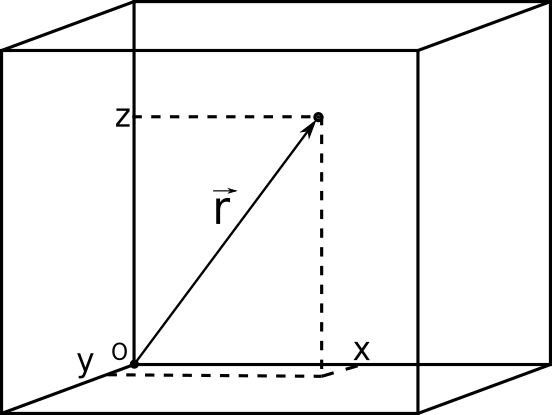
\includegraphics[scale=1]{img/vecr.png}
    
    \caption{\footnotesize Coordenadas de $P$ determinadas por $\vec{r}$.}

    \label{vecr}
\end{staticfigure}

\subsubsection*{Deslocamento}
O deslocamento $(\Delta \vec{r})$ de $P$ pode ser entendido como:

\begin{mydef}
    É definido como deslocamento $(\Delta \vec{r})$ de $P$, qualquer variação 
    no vetor posição $(\vec{r})$ ocorrida ao longo do tempo.
\end{mydef}

onde $(\Delta \vec{r})$ é definido como:

\begin{equation}
    \Delta \vec{r} = \vec{r}(t + \Delta t ) - \vec{r}(t)
\end{equation}

No estudo da Cinemática Retilinear, devido aos movimentos serem sempre 
unidirecionais, é comum que seja adotada a notação escalar das grandezas, ou 
seja, a magnitude do vetor posição e quaisquer deslocamentos sofridos por 
ele podem ser obtidos algebricamente, já suas coordenadas podem ser 
representadas por um escalar $s$.

Esta convenção admite a seguinte propriedade:

\begin{proof}
Considerando que:
$$
\left |\vec{r} \right | = \sqrt{(x^2 + y^2 + z^2)}
$$

e que $x=s$, $y=0$ e $z=0$ então; 

$$
\left |\vec{r} \right | = \sqrt{(s^2)}
$$

e que, 

$$
\left |\vec{r} \right | = s
$$

\end{proof}
Por conseguinte, o deslocamento retilinear pode ser determinado por:

\begin{equation}
    \Delta s = s( t + \Delta t ) - s(t)
\end{equation}

\section{Grandezas Cinemáticas}

A Cinemática, como parte da Mecânica que se ocupa da descrição espacial do 
movimento, se baseia em três grandezas básicas. A posição, 
já descrita na seção anterior, é a primeira delas, as demais são a 
velocidade $\vec{v}$ e a aceleração $\vec{a}$.

\subsection{Velocidade}

Na Cinemática a velocidade é tratada de duas formas distintas;
como velocidade média e velocidade instantânea ou simplesmente velocidade. 

\subsubsection*{Velocidade Média}
Quando um Ponto Material $P$, translada de uma posição $\vec{r}$, para uma 
posição $\vec{r'}$ durante um intervalo de tempo $\Delta t$, então a velocidade
média pode ser obtida conforme o mostrado na Eq. \ref{v_med}.

\begin{equation}
    \vec{v}_{med} = \frac{\Delta \vec{r}}{\Delta t}
    \label{v_med}
\end{equation}

Onde, $\Delta \vec{r}$ é o deslocamento e $\Delta t$ o intervalo de tempo 
transcorrido durante o deslocamento, conforme mostrado na Fig. \ref{vmed}.

\begin{staticfigure}
    \centering
    
    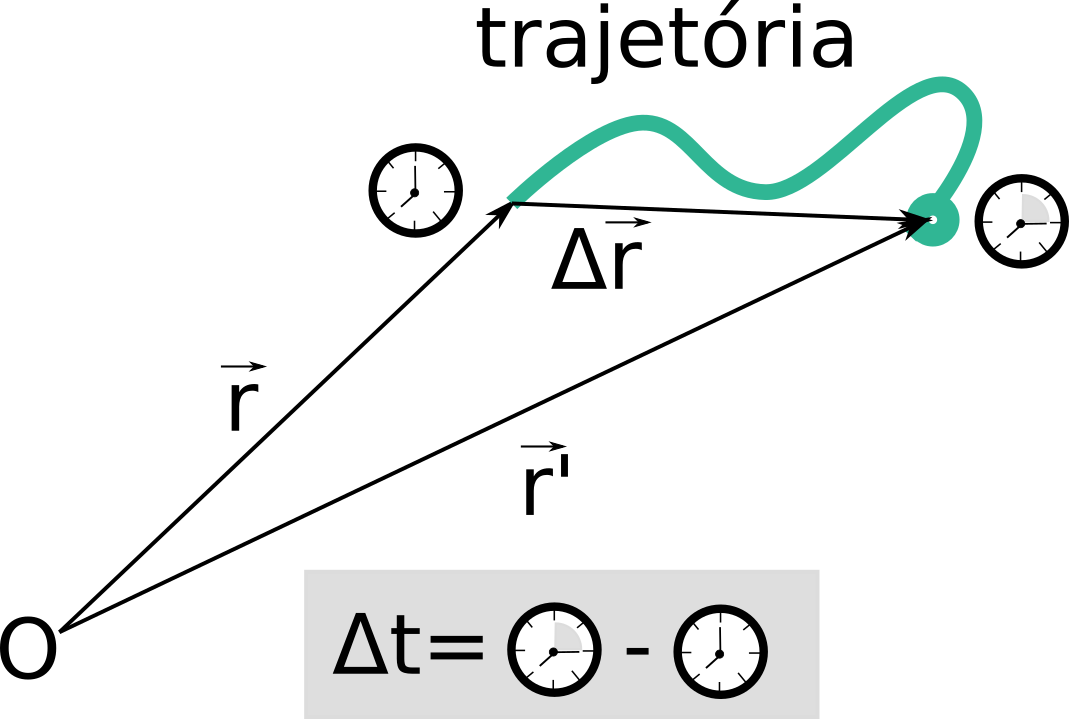
\includegraphics[scale=0.5]{img/vmed.png}

    \caption{\footnotesize Descrição visual do conceito de velocidade média.}
    \label{vmed}

\end{staticfigure}

Ocasionalmente pode interessar a determinação da velocidade média ao longo da 
trajetória de comprimento $s_T$. Nestes casos, define-se a velocidade média de 
percurso como $v_{perc}$, que é uma grandeza escalar definida pela Eq. 
\ref{vperc}.

\begin{equation}
    \left( v_{perc} \right)_{med} = \frac{s_T}{\Delta t}
    \label{vperc}
\end{equation}

Onde $s_T$ é comprimento da trajetória percorrida por $P$.



\subsubsection*{Velocidade Instantânea}
Quando o intervalo de tempo considerado para a determinação da velocidade 
média diminui gradativamente, o deslocamento tende a zero e a valor da 
velocidade média tende para o valor da velocidade instantânea, conforme mostrado na 
Fig. \ref{vinst} e a Eq. \ref{eq_vinst}.

\begin{equation}
\vec{v}(t) = \lim_{\Delta t\rightarrow 0} \frac{\Delta \vec{r}}{\Delta t} = 
\frac{d \vec{r}}{d t}
\label{eq_vinst}
\end{equation}

\begin{staticfigure}
    \centering

    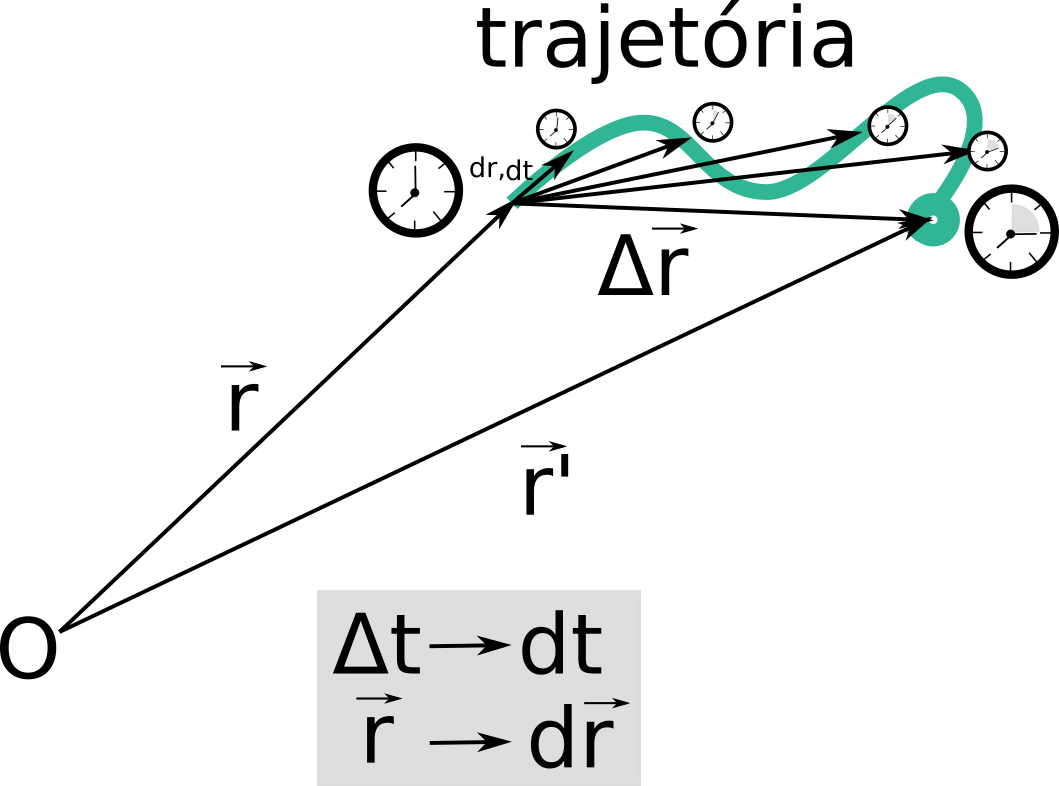
\includegraphics[scale=0.5]{img/vinst.png}

    \caption{\footnotesize Descrição visual do conceito de velocidade instantânea.}
    \label{vinst}
\end{staticfigure}

Por conseguinte a velocidade de um corpo é definida como:

\begin{mydef}
    Velocidade é a taxa temporal de variação da posição de um corpo.
\end{mydef}

Como a  Eq. \ref{eq_vinst} mostra a velocidade como taxa de variação da 
posição, pode interessar, em casos como estes, que, a partir da velocidade 
dada como função do tempo, se obtenha a função horária da posição. 
O método para tal consiste na obtenção da antiderivada de $v(t)$, conforme 
mostrado abaixo. Por motivo de simplificação matemática, considere o caso 
retilinear.

$$
v(t) = \frac{d s}{dt} \rightarrow 
\int_{s(t)}^{s(t+\Delta t)}ds = \int_{t}^{t+\Delta t}{v(t) dt}
$$


Considerando as condições iniciais arbitradas como $t=0$ e $s(t=0)=0$, então
a relação anterior pode ser escrita na forma da Eq. \ref{eq_int_pos}, onde 
a posição inicial $s(0)$ é a constante adicionada na integração definida.

\begin{equation}
    s(t) = \left( \int_{0}^{t} v(t) dt \right) + s(0)
    \label{eq_int_pos}
\end{equation}

\subsection{Aceleração}
Assim como a velocidade, a aceleração pode ser tratada de duas formas 
distintas, como aceleração média e instânea. A lógica para obtenção de cada uma
das grandezas é semelhante àquela utilizada para a velocidade. 

\subsubsection*{Aceleração Média}
A aceleração média de um corpo é definida como razão entre a variação da 
velocidade e o intervalo de tempo transcorrido durante esta variação, conforme
mostrado na Eq. \ref{acel_med}.

\begin{equation}
    \vec{a}_{med} = \frac{\Delta \vec{v}}{\Delta \vec{t}}
    \label{acel_med}
\end{equation}

\subsubsection*{Aceleração Instantânea}
A aceleração instante, ou simplesmente aceleração é definida como se segue:

\begin{mydef}
    A aceleração é definida como a taxa temporal de variação da velocidade 
    conforme mostrado na Eq. \ref{eq_ainst}. 
\end{mydef}

\begin{equation}
    \vec{a}(t) = \lim_{\Delta t\rightarrow 0} \frac{\Delta \vec{v}}{\Delta t} = 
    \frac{d \vec{v}}{d t}
    \label{eq_ainst}
\end{equation}

Como consequência direta da Eq. \ref{eq_ainst}, pode-se provar que:

\begin{proof}
Se $v = \frac{ds}{dt}$ e $a = \frac{dv}{dt}$, então a primeira equação pode 
ser substituída na segunda da seguinte forma:

\begin{equation}
a = \frac{d\left( \frac{ds}{dt}\right)}{dt} = \frac{d^2 s}{dt^2}
\end{equation}

\end{proof}

Assim como demonstrado para a Eq. \ref{eq_int_pos}, a função $v(t)$ pode 
ser obtida pela integração de $a(t)$, conforme mostra a demonstração:

$$
a(t) = \frac{d v}{dt} \rightarrow 
\int_{v(t)}^{v(t+\Delta t)} dv = \int_{t}^{t+\Delta t} a(t) dt
$$


Considerando a condição inicial arbitrada como $t=0$, então
a relação anterior pode ser escrita na forma da Eq. \ref{eq_int_pos}.

\begin{equation}
    v(t) = \int_{0}^{\Delta t} a(t) dt
    \label{eq_int_pos_}
\end{equation}

\begin{myboxed}
    \textbf{EXEMPLO - Determinando a aceleração e o deslocamento a partir da
    velocidade de um corpo. .}

    Uma partícula (ponto material), desloca-se retilinearmente segundo a função
    horário $v(t) = (8,0.t^2-4,0t)m.s^{-1}$. Determine \emph{a)} sua velocidade 
    inicial; \emph{b)} seu deslocamento $\Delta s$ em $10 \: s$ de movimento e 
    \emph{c)} a função horária da aceleração. 

    \textbf{SOLUÇÃO:}

    \emph{a)} A velocidade inicial é definida como aquela ocorrida em $t=0$, 
    logo $v(0)$ que pode ser determinada como:
    
    $$
        v(0) = 8,0\:.\:0^2 - 4,0\:.\:0 = 0,0 m.s^{-1}
    $$

    \emph{b)} O deslocamento pode ser obtido fazendo-se a integral definida no 
    intervalo considerado, conforme mostrado na Equação \ref{eq_int_pos}, 
    porém, como a posição inicial é desconhecida, o problema exige apenas o 
    cálculo do deslocamento $\Delta s = s(t) - s(0)$, conforme se segue:

    $$
    \Delta s = \int_0^{10} (8,0t^2-4,0\:t) dt = \left[ \frac{8,0}{3} t^3 - 2,0 t^2\right]_0^{10} = \frac{7,4 \: . \: 10^3}{ 3} \: m
    $$

    \emph{c)} Já a função horária da aceleração, é obtida por meio da primeira 
    derivada temporal de $v(t)$, conforme segue:

    $$
    a(t) = \frac{d((8,0.t^2-4,0t))}{dt} = (16,0 t - 4) m.s^{-2}
    $$

\end{myboxed}

\subsection{Relação Diferencial entre $v(t)$ e $s(t)$}
Sabendo que tanto a posição quanto a velocidade são funções do tempo, 
podemos, baseados no Cálculo, a priori, supor que possa existir uma função 
composta por ambas $v \circ s$. 

Mas por que não o contrário? Por motivos físicos principalmente, é mais 
razoável supor uma função de velocidade dependente da posição, do que uma 
posição dependente da velocidade, já que a posição pode ser interpretada 
como uma grandeza fundamental e a velocidade só pode ser entendida como 
uma grandeza derivada.

A composição ($v \circ s$) sugerida, pode ser matematicamente realizada, 
dentre outras formas menos rigorosas, principalmente por meio da regra da cadeia 
que diz - para este caso - que se $v$ é diferenciável em $s$, então esta 
derivada pode ser obtida pelo produto da derivada de $v$ em $u$ pela 
derivada de $u$ em $s$, onde, por conveniência, $u=t$, ou seja:

$$
\frac{dv}{ds} = \frac{dv}{du} \cdot \frac{du}{ds} = \frac{dv}{dt} \cdot \frac{dt}{ds}
$$

Após a aplicação da regra, pode-se notar que o primeiro fator do produto das 
derivadas $\frac{dv}{dt}$ é a própria definição de aceleração, enquanto o 
segundo fator $\frac{dt}{ds}$ é o inverso da definição de velocidade, ou seja, 
$\frac{1}{v}$, podendo a equação ser escrita na forma dada em Eq. \ref{rel_dif}.

\begin{equation}
    \frac{dv}{ds} = a \cdot \frac{1}{v} \rightarrow v \cdot dv = a \cdot ds
    \label{rel_dif}
\end{equation}

\begin{myboxed}
    \textbf{EXEMPLO - Atração magnética em meio viscoso.}

    Uma partícula ferromagnética está submetida à influência de um campo magnético
    conforme ela se move para baixo em um fluído que preenche o espaço entre 
    as placas A e B da figura. O ponto material, que incialmente estava em repouso, 
    foi abandonado, em uma posição equidistante do centro das placas à 100 mm de 
    cada uma delas. Seu movimento dá-se com aceleração $a(s) = (4s) m.s^{-2}$. 
    Determine a velocidade com que ele atinge a placa B, assim como o tempo de 
    movimento. 

    \begin{staticfigure}
        \centering
        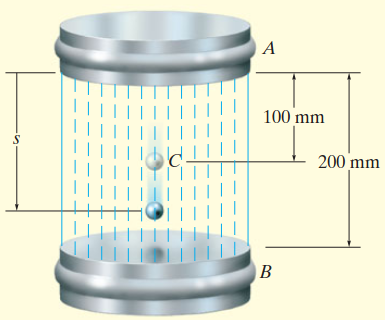
\includegraphics[scale=0.4]{img/hibbelerexerc.png}
        \caption{Adaptado de Hibbeler.}
    \end{staticfigure}

    \textbf{SOLUÇÃO:}

    É notável que a função da aceleração $a(s)$, tem sinal positivo, sugerindo 
    um aumento da aceleração à medida que a partícula progride na trajetória. 
    É igualmente notável que o movimento é descendente, já que o objetivo de
    cálculo dá-se na placa B a partir do ponto C. Devido a essas peculiaridades 
    do enunciado, adotaremos o sentido $A \rightarrow B$ como positivo para a 
    análise. 

    Aplicando a relação diferencial \ref{rel_dif}, para a solução e a devidas 
    conversões de unidade pode-se fazer:

    $$
    v dv = a ds 
    \rightarrow \int_0^{v} v dv = \int_{0,10 \: m}^{s(t)} {4s \: ds}
    $$

    $$
    \frac{1}{2} v^2 = \left[ \frac{4}{2} s^2 \right]_{0,10}^{s(t)} \rightarrow
    v(s) = 2\sqrt{s^2 - 0,01},
    $$

    que para 0,20 m (200 mm entre A e B), resulta em: \emph{continua...}
\end{myboxed}
\begin{myboxed}
    $$
    v(0,20 \: m) \approx 0,346 \: m/s,
    $$

    onde a raiz positiva foi escolhida pois, como dito, este é o sentido 
    convencionado para o movimento. 

    Conhecida a velocidade $v(s) = 2\sqrt{s^2 - 0,01}$, pode-se utilizar sua 
    definição $v = ds / dt$, para a determinação do tempo de movimento. 

    $$
    v = \frac{ds}{dt} \rightarrow \frac{ds}{v} =  dt \rightarrow 
    \int_{0,10}^{s(t)} \frac{ds}{(2\sqrt{s(t)^2 - 0,01})} = \int_0^t { dt},
    $$

    cuja solução é:

    $$
    ln(\sqrt{s(t)^2 - 0,01} + s(t))_{0,10}^{s(t)} = 2t \rightarrow
    ln(\sqrt{s(t)^2 - 0,01} + s(t)) + 2,33 \approx 2t
    $$
    
    que substituindo $s(t) = 0,20 m$ resulta em $t \approx 0,658 s$. 

    Consulte sua tabela de integrais caso haja dúvida no processo de integração.

    
\end{myboxed}

\subsection{Caso Especial: O Movimento com Aceleração Constante}

Em alguns fenômenos e idealizações, um comportamento peculiar pode ser
observado, a ocorrência de aceleração constante. Provavelmente, o fenômeno deste 
tipo mais amplamente conhecido é a queda livre.

\begin{mydef}
    A queda livre é um tipo de movimento sobre o qual atua exclusivamente a 
    força gravitacional ($F_G$), por isso é uma idealização, já que quaisquer
    outras interferências dinâmicas devem ser desprezadas. 
\end{mydef}

De forma generalizada, para se compreender o movimento com aceleração constante,
deve-se partir da Equação \ref{eq_ainst} admitindo que que 
$\frac{d \vec{v}}{dt} = k$ e que $k$ é uma aceleração constante, $k = \vec{a}$.

Deste modo, podemos determinar a função horária da velocidade em um movimento 
deste tipo. \emph{As funções horárias de velocidade, são funções capazes de 
determinar o vetor velocidade como função exclusiva do tempo, endo escritas na
forma} $y = v(t)$. 

\begin{proof}
    \label{Dem:func_h_vel}
    Se:
    $$
    a_{const} = \frac{dv}{dt},
    $$
    onde o caráter vetorial foi propositalmente omitido por tratar-se de 
    cinemática retilinear; então se pode fazer antiderivação da seguinte forma:

    $$
        dv = a \: . \: dt \rightarrow 
        \int_{v(t=0)}^{v(t+\Delta t)} (dv) = \int_{t=0}^{t+\Delta t} (a \: . \: dt),
    $$
    onde o limite inferior foi assumido como ($t=0$) e que resulta em:

    $$
    \Delta v = a\: . \:t,
    $$

    Finalmente dando origem a Equação \ref{Eq:func_hor_vel_ak}.
    
    \begin{equation}
        v(t) = a\: . \:t + v(0)
        \label{Eq:func_hor_vel_ak}
    \end{equation}

    Onde $v(t)$ é a velocidade no tempo $t > 0$, $a$ a aceleração constante e 
    $v(0)$, a velocidade inicial.
\end{proof}

Para a posição $s(t)$, ou $\vec{r}(t)$ \footnote{Em nosso curso geralmente 
utilizaremos $s$ para denotar a posição como uma grandeza escalar e $\vec{r}$
para representar a posição como uma grandeza vetorial.}, deve-se repetir o 
mesmo procedimento da Demonstração \ref{Dem:func_h_vel} no entanto, partindo da
Equação \ref{eq_int_pos}.

\begin{proof}
    Se $s(t) = \int_{0}^{t} v(t) dt$ e $v(t) = a\: . \:t + v(0)$, então:

    $$
        s(t) = \left(\int_{0}^{t} (a\: . \:t + v(0)) dt \right) + s(0),
    $$

    resultando na forma da \textbf{função horária da posição} dada pela 
    Equação \ref{Eq:func_hr_pos}.

    \begin{equation}
        s(t) =  \frac{1}{2} a \: . \: t^2 + v(0)\: . \: t + s(0);
        \label{Eq:func_hr_pos}
    \end{equation}

\end{proof}

Uma terceira ferramenta, muito utilizada em casos onde a aceleração do movimento 
retilinear, é constante é a Equação de Torricelli dada pela Equação 
\ref{Eq:Torricelli}. Veja sua demonstração. 
\begin{proof}

    Tomando $t$ na função horária da velocidade, na forma 
    $t = \frac{v(t) - v(0)}{a}$, e substituindo o seu valor na Equação 
    \ref{Eq:func_hr_pos}. 

    Pode-se fazer:

    $$
    i) \: s(t) = s(0) + v(0) \frac{v(t) - v(0)}{a} + \frac{1}{2} a \left(\frac{v(t) - v(0)}{a} \right)^2
    $$
    $$
    ii) \: s(t) = s(0) + v(0) \frac{v(t) - v(0)}{a} + \frac{1}{2} a \left(\frac{v(t) - v(0)}{a} \right)^2
    $$
    $$
    iii) \: s(t) = s(0) +  \frac{v(t)v(0) - v(0)^2}{a} + \frac{1}{2} a \left(\frac{v(t)^2 - 2v(t)v(0) + v(0)^2}{a a} \right)
    $$
    $$
    iv) \: s(t) - s(0) =  \frac{v(t)v(0) - v(0)^2}{a} + \left(\frac{v(t)^2 - 2v(t)v(0) + v(0)^2}{2a} \right)
    $$
    $$
    v) \: s(t) - s(0) = \frac{2v(t)v(0) - 2v(0)^2 + v(t)^2 - 2v(t)v(0) + v(0)^2}{2a}
    $$
    $$
    vi) \: s(t) - s(0) = \frac{2v(t)v(0) - 2v(0)^2 + v(t)^2 - 2v(t)v(0) + v(0)^2}{2a}
    $$
    $$
    vii) \: \Delta s = \frac{ -v(0)^2 + v(t)^2  }{2a} \rightarrow  2a \Delta s=  -v(0)^2 + v(t)^2
    $$
    
    \begin{equation}
        \label{Eq:Torricelli}
        v(t)^2 = v(0)^2 + 2 a \Delta s
    \end{equation}
\end{proof}

Uma demonstração mais simples e, simultaneamente, mais rigorosa, poderia ser 
obtida da Equação \ref{rel_dif}, conforme demonstrado abaixo. 

\begin{proof}
    $$
    v \cdot dv = a \cdot ds \rightarrow 
    \int_{v(0)}^{v(t)} v \cdot dv =  \int_{s(0)}^{s(t)} a \cdot ds
    $$

    $$
    \frac{v(t)^2 - v(0)^2}{2} = a (s(t) - s(0)) \rightarrow v(t)^2 - v(0)^2 = 2 a \Delta s
    $$

    resultando na forma da Equação \ref{rel_dif}

    $$
    v(t)^2 = v(0)^2 + 2 a \Delta s
    $$
\end{proof}

Uma importante característica da Equação de Torricelli é que é independente do 
tempo, de forma tal que velocidades, acelerações e deslocamentos podem ser 
obtidos para situações onde esta grandeza for omitida ou desconhecida.

Ainda que a Equação \ref{Eq:Torricelli} seja válida exclusivamente para casos com 
aceleração constante, a relação expressa pela Equação \ref{rel_dif}, não o é, 
podendo ser aplicada de forma generalizada.

Devido ao algebrismo próprio do movimento com aceleração constante ser muito 
elementar e idêntico à abordagem comum utilizada durante o ensino médio, não 
serão oferecidos exemplos de uso das equações nesta subseção. 

\label{lastpage}
\end{document}